\documentclass[11pt]{article}
\usepackage[a4paper,margin=2.3cm]{geometry}
\usepackage{amsmath,amssymb,bm}
\usepackage{booktabs,array}
\usepackage{enumitem}
\usepackage[dvipsnames]{xcolor}
\usepackage[most]{tcolorbox}
\usepackage{tikz}
\usetikzlibrary{positioning,arrows.meta,backgrounds,decorations.pathreplacing,shapes.geometric}
\usepackage{microtype}
\usepackage[colorlinks=true,linkcolor=NavyBlue,urlcolor=NavyBlue]{hyperref}

\newtcolorbox{keybox}[1][]{colback=Gray!6,colframe=Gray!55,boxrule=0.5pt,
  arc=2pt,left=6pt,right=6pt,top=5pt,bottom=5pt,#1}
\newtcolorbox{warnbox}[1][]{colback=BrickRed!5,colframe=BrickRed!60,boxrule=0.6pt,
  arc=2pt,left=6pt,right=6pt,top=5pt,bottom=5pt,#1}
\newtcolorbox{goodbox}[1][]{colback=ForestGreen!6,colframe=ForestGreen!55,boxrule=0.6pt,
  arc=2pt,left=6pt,right=6pt,top=5pt,bottom=5pt,#1}

\newcommand{\ula}{\textcolor{NavyBlue}{\textbf{ULA}}}
\newcommand{\eca}{\textcolor{BrickRed}{\textbf{ECA}}}
\newcommand{\cape}{\textbf{CAPE}}

\title{\textbf{Sparse Arrays for Near-Field Cell-Free XL-MIMO}\\[3pt]
\large Crowded vs.\ Uncrowded Users, the Proposed CAPE Technique,\\
and How It Differs from Existing Sparse-Array Methods}
\author{Explanatory note (simple English)}
\date{\today}

\begin{document}
\maketitle

\begin{keybox}
\textbf{What this document answers, in plain words.}
\begin{enumerate}[leftmargin=1.4em,itemsep=1pt]
\item Are your 8 users ``crowded''? What do crowded and uncrowded mean?
\item Why does crowding matter? Who benefits from the sparse array, and who does not?
\item How are antennas arranged in old arrays (ULA, uniform sparse, ECA), and does the
      proposed method ``stretch'' the array in a new way?
\item How is the proposed technique different from the 2025 ECA paper? What exactly is new?
\item The full working of the proposed system, step by step, from the antennas to the user.
\end{enumerate}
\end{keybox}

%====================================================================
\section{The short answer first}

\begin{keybox}
\textbf{Your current scenario (8 users spread over the 300$\times$300\,m area) is the
\emph{uncrowded} case.} This is exactly the case where the proposed technique only
\emph{ties} the old dense array. The proposed technique shows a clear gain only when the
users become \emph{crowded} (many users close together in a small spot).
\end{keybox}

Two more things to fix in your mental picture before the details:

\begin{itemize}[leftmargin=1.4em,itemsep=2pt]
\item \textbf{The proposed method does \emph{not} invent a new antenna layout.} It uses the
      same ECA (extended co-prime array) layout from the 2025 paper. We do \emph{not}
      ``stretch the array in a new way''.
\item \textbf{What is new is the \emph{signal processing}, not the array.} The new part is how
      several access points (APs) \emph{cooperate} to estimate the channel of a sparse array.
      We call it \cape{} (Cross-AP Position-fused Estimation). This is the honest novelty, and
      it is what makes the sparse array actually useful in a cell-free network.
\end{itemize}

%====================================================================
\section{What ``crowded'' and ``uncrowded'' users mean}

Picture the service area as a 300\,m $\times$ 300\,m square. There are $L=8$ access points
(APs) placed around it, and $K=8$ users somewhere inside it.

\begin{center}
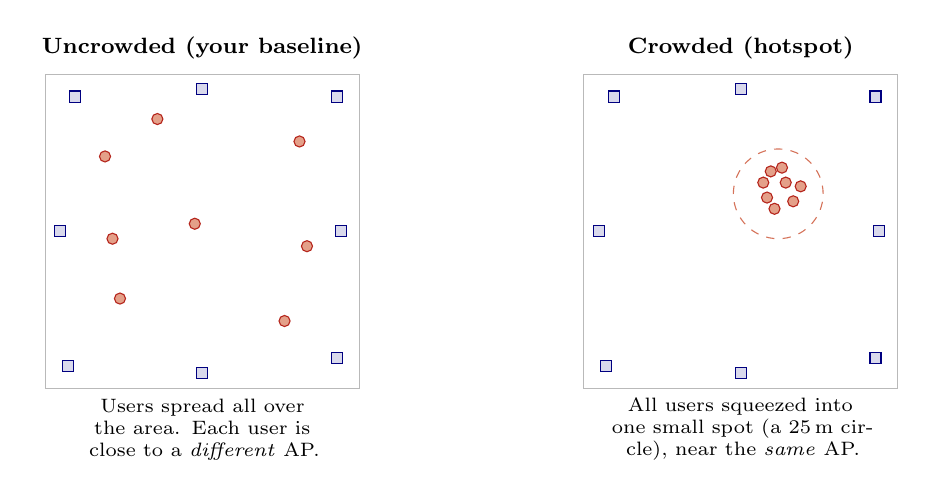
\begin{tikzpicture}[scale=0.95,
  ap/.style={rectangle,draw=NavyBlue,fill=NavyBlue!15,minimum size=4pt,inner sep=2pt},
  ue/.style={circle,draw=BrickRed,fill=BrickRed!35,minimum size=4pt,inner sep=1.3pt}]
% ---- left: uncrowded ----
\begin{scope}
  \draw[Gray!55] (0,0) rectangle (4.2,4.2);
  \node[font=\footnotesize\bfseries] at (2.1,4.55) {Uncrowded (your baseline)};
  \foreach \x/\y in {0.3/0.3, 3.9/0.4, 0.4/3.9, 3.9/3.9, 2.1/0.2, 0.2/2.1, 3.95/2.1, 2.1/4.0}
     \node[ap] at (\x,\y) {};
  \foreach \x/\y in {1.0/1.2, 3.2/0.9, 0.8/3.1, 3.4/3.3, 2.0/2.2, 1.5/3.6, 3.5/1.9, 0.9/2.0}
     \node[ue] at (\x,\y) {};
  \node[font=\scriptsize,text width=4.2cm,align=center] at (2.1,-0.55)
     {Users spread all over the area. Each user is close to a \emph{different} AP.};
\end{scope}
% ---- right: crowded ----
\begin{scope}[xshift=7.2cm]
  \draw[Gray!55] (0,0) rectangle (4.2,4.2);
  \node[font=\footnotesize\bfseries] at (2.1,4.55) {Crowded (hotspot)};
  \foreach \x/\y in {0.3/0.3, 3.9/0.4, 0.4/3.9, 3.9/3.9, 2.1/0.2, 0.2/2.1, 3.95/2.1, 2.1/4.0}
     \node[ap] at (\x,\y) {};
  \draw[BrickRed!55,dashed] (2.6,2.6) circle (0.6);
  \foreach \x/\y in {2.45/2.55, 2.7/2.75, 2.55/2.4, 2.8/2.5, 2.4/2.75, 2.65/2.95, 2.9/2.7, 2.5/2.9}
     \node[ue] at (\x,\y) {};
  \node[font=\scriptsize,text width=4.2cm,align=center] at (2.1,-0.55)
     {All users squeezed into one small spot (a 25\,m circle), near the \emph{same} AP.};
\end{scope}
\end{tikzpicture}
\end{center}

\begin{description}[leftmargin=0pt,itemsep=4pt]
\item[\textcolor{ForestGreen}{\textbf{Uncrowded (``baseline'' in the code).}}] Users are spread
  across the whole area. In the code each user is dropped around a different AP, at a distance
  of 20--150\,m. Because they sit in different directions and different distances, \emph{the
  network can already tell them apart easily}. \textbf{This is your current 8-user setup.}
\item[\textcolor{BrickRed}{\textbf{Crowded (``hotspot'' in the code).}}] All users sit inside one
  small circle (radius 25\,m by default; the sweep also tries 10\,m, which is very crowded). A
  real example: everyone in one lecture hall, one stadium stand, one train platform, one
  conference room. To a nearby AP, all these users arrive from nearly the \emph{same direction}
  and nearly the \emph{same distance}, so \emph{their radio channels look almost identical}.
\end{description}

\begin{keybox}
\textbf{The one-line definition.} Users are \emph{crowded} when their channels look similar to
an AP (same direction, similar distance), so the AP struggles to separate them. They are
\emph{uncrowded} when their channels look different, so separation is easy.
\end{keybox}

%====================================================================
\section{Why crowding decides who benefits}

A big antenna array is a tool for \emph{separating} users in space. If the users are already
easy to separate, a better tool does not help. If the users are hard to separate, a better tool
helps a lot. That is the whole story.

\begin{center}
\renewcommand{\arraystretch}{1.25}
\begin{tabular}{@{}p{3.1cm}p{5.6cm}p{5.6cm}@{}}
\toprule
 & \textcolor{ForestGreen}{\textbf{Uncrowded users}} & \textcolor{BrickRed}{\textbf{Crowded users}}\\
\midrule
Do their channels look alike? & No. Different directions / distances. & Yes. Nearly the same.\\
Can the network separate them already? & Yes, easily (many APs see them differently). & No, this is the hard part.\\
Does extra array resolution help? & \textbf{Almost not at all.} The job is already done. & \textbf{Yes, a lot.} This is the bottleneck.\\
So the sparse array\dots & \dots gives no real gain (a tie). & \dots gives a clear gain.\\
\bottomrule
\end{tabular}
\end{center}

\begin{keybox}
\textbf{Why ``should'' users be crowded for the gain to appear?} It is not that crowding is good
for the users --- crowding is actually a hard, stressful situation for the system (lots of mutual
interference). It is that \emph{crowding is the situation where a better array earns its keep}. A
sharper tool only shows its value on a hard job. When the job is easy (uncrowded), any tool looks
the same, so the sparse array and the dense array tie. When the job is hard (crowded), the sparse
array's extra resolution finally matters, and the proposed technique wins.
\end{keybox}

This is exactly what your results showed (the crowding-sweep figure): as the hotspot radius
shrinks from 200\,m down to 10\,m, the proposed curve pulls further and further below the dense
array. At 10\,m the proposed technique had about 2.5--4$\times$ lower bit-error rate; at 100\,m
they met.

%====================================================================
\section{How antennas are arranged: dense, uniform-sparse, ECA}

All of these use the \emph{same number} of antennas ($N\approx64$). The only difference is
\emph{where} the antennas sit. ``Stretching'' the array means spreading the same antennas over a
wider line, which gives a bigger aperture and sharper resolution --- but spreading them wrongly
creates ghost beams (grating lobes).

\begin{center}
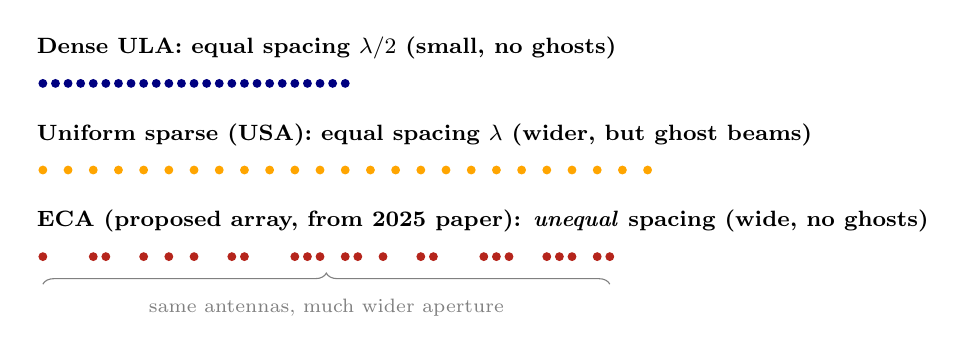
\begin{tikzpicture}[scale=1.0,dot/.style={circle,fill=#1,minimum size=3.2pt,inner sep=0pt}]
% ULA
\node[font=\footnotesize\bfseries,anchor=west] at (-0.2,2.55) {Dense ULA: equal spacing $\lambda/2$ (small, no ghosts)};
\foreach \i in {0,...,24} \node[dot=NavyBlue] at ({\i*0.16},2.1) {};
% USA
\node[font=\footnotesize\bfseries,anchor=west] at (-0.2,1.45) {Uniform sparse (USA): equal spacing $\lambda$ (wider, but ghost beams)};
\foreach \i in {0,...,24} \node[dot=Orange] at ({\i*0.32},1.0) {};
% ECA
\node[font=\footnotesize\bfseries,anchor=west] at (-0.2,0.35) {ECA (proposed array, from 2025 paper): \emph{unequal} spacing (wide, no ghosts)};
\foreach \p in {0,0.64,0.8,1.28,1.6,1.92,2.4,2.56,3.2,3.36,3.52,3.84,4.0,4.32,4.8,4.96,5.6,5.76,5.92,6.4,6.56,6.72,7.04,7.2}
   \node[dot=BrickRed] at (\p,-0.1) {};
\draw[decorate,decoration={brace,amplitude=4pt},Gray] (0,-0.45) -- (7.2,-0.45)
   node[midway,below,font=\scriptsize,yshift=-2pt]{same antennas, much wider aperture};
\end{tikzpicture}
\end{center}

\begin{center}
\renewcommand{\arraystretch}{1.2}
\begin{tabular}{@{}lcccp{4.3cm}@{}}
\toprule
Array & Spacing & Aperture & Ghost beams & Note\\
\midrule
\ula{} (dense)        & equal, $\lambda/2$ & small (3.15\,m) & none & poor range resolution\\
USA (uniform sparse)  & equal, $\lambda$   & wide (6.3\,m)   & \textbf{strong} & ghosts cause confusion\\
\eca{} (non-uniform)  & \textbf{unequal}   & widest (7.6\,m) & none (suppressed) & weak scattered sidelobes\\
\bottomrule
\end{tabular}
\end{center}

\begin{description}[leftmargin=0pt,itemsep=3pt]
\item[\textbf{ULA (old, dense).}] You ``stretch'' nothing: antennas are packed at half a
  wavelength. The array is short, so it cannot focus in \emph{distance} well; two users on the
  same line (one near, one far) look almost identical.
\item[\textbf{USA (old, uniform sparse).}] You ``stretch'' the array \emph{uniformly}: keep equal
  spacing but make it larger. The array is now wide and sharp, \emph{but} equal spacing creates
  exact copies of the beam at other angles --- \emph{grating lobes} (ghost beams). A user sitting
  on a ghost beam is confused with the real one.
\item[\textbf{ECA (the array we use, from the 2025 paper).}] You ``stretch'' the array
  \emph{non-uniformly}: antennas sit at \emph{unequal} gaps following a co-prime pattern. Because
  the gaps are irregular, the ghost copies never line up, so there are no strong ghost beams. The
  price is a floor of weak scattered sidelobes.
\end{description}

\begin{keybox}
\textbf{So does the proposed method stretch the array?} It uses the ECA stretch --- non-uniform,
wide, no strong ghosts. \textbf{We do not change how a \emph{single} array is stretched.} Our new
idea works at the \emph{network} level, across many APs, and is described next.
\end{keybox}

%====================================================================
\section{What is actually new: the CAPE technique}

A sparse array has one weakness: it is \emph{ambiguous}. Its beam is very sharp, but it also has
several ``maybe'' spots where a user could be. One AP alone cannot always tell the true spot from
the false ones --- this is what hurt the plain ECA and made its channel estimates worse than the
dense ULA.

\begin{keybox}
\textbf{Key idea of CAPE (one sentence).} A user has only \emph{one} true physical location, and
every AP's channel is a known function of that location; so if we \emph{combine} the sparse
arrays of several APs, the true location is the only spot they all agree on --- the false spots of
one AP are killed by the others.
\end{keybox}

\begin{center}
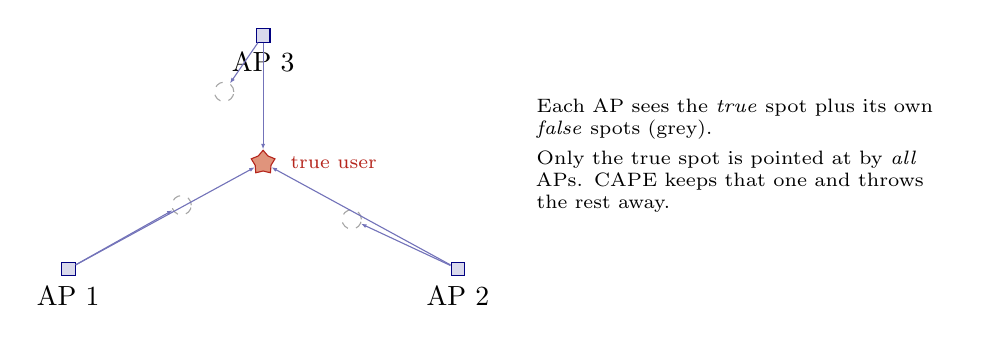
\begin{tikzpicture}[scale=0.9,
  ap/.style={rectangle,draw=NavyBlue,fill=NavyBlue!15,minimum size=5pt,inner sep=2pt},
  ue/.style={star,star points=5,draw=BrickRed,fill=BrickRed!40,minimum size=9pt,inner sep=0.5pt},
  ghost/.style={circle,draw=Gray!70,dashed,minimum size=7pt,inner sep=0pt}]
\node[ap,label=below:{AP 1}] (a1) at (0,0) {};
\node[ap,label=below:{AP 2}] (a2) at (5.5,0) {};
\node[ap,label=below:{AP 3}] (a3) at (2.75,3.3) {};
\node[ue] (u) at (2.75,1.5) {};
\node[font=\scriptsize,BrickRed,anchor=west] at (3.0,1.5) {true user};
% ghosts (each AP has its own false spots)
\node[ghost] (g1) at (1.6,0.9) {};
\node[ghost] (g2) at (4.0,0.7) {};
\node[ghost] (g3) at (2.2,2.5) {};
\draw[NavyBlue!55,-{Latex[length=2pt]}] (a1) -- (u);
\draw[NavyBlue!55,-{Latex[length=2pt]}] (a1) -- (g1);
\draw[NavyBlue!55,-{Latex[length=2pt]}] (a2) -- (u);
\draw[NavyBlue!55,-{Latex[length=2pt]}] (a2) -- (g2);
\draw[NavyBlue!55,-{Latex[length=2pt]}] (a3) -- (u);
\draw[NavyBlue!55,-{Latex[length=2pt]}] (a3) -- (g3);
\node[font=\scriptsize,text width=5.2cm,align=left] at (9.5,1.6)
 {Each AP sees the \emph{true} spot plus its own \emph{false} spots (grey).\\[3pt]
  Only the true spot is pointed at by \emph{all} APs. CAPE keeps that one and
  throws the rest away.};
\end{tikzpicture}
\end{center}

\subsection*{How CAPE differs from the 2025 ECA paper}

\begin{center}
\renewcommand{\arraystretch}{1.25}
\begin{tabular}{@{}p{4.1cm}p{5.0cm}p{5.0cm}@{}}
\toprule
 & \textbf{2025 ECA paper (Zhou \emph{et al.})} & \textbf{This work (proposed)}\\
\midrule
Array geometry & ECA (they proposed it) & \textbf{Same ECA (we reuse it, we cite them)}\\
How many arrays & \textbf{One} array / base station & \textbf{Many} APs (cell-free, $L=8$)\\
Direction & Downlink (transmit beamforming) & \textbf{Uplink} (receive / data detection)\\
Main contribution & Beam-pattern analysis, hybrid beamforming for one array & \textbf{CAPE: APs cooperate to remove the sparse array's ambiguity in channel \emph{estimation}}\\
Ambiguity handling & Analysed for a single array & \textbf{Removed by fusing several APs}\\
Detector & --- & Cross-AP list SIC (your earlier work)\\
\bottomrule
\end{tabular}
\end{center}

\begin{warnbox}
\textbf{Be honest in the paper.} Do \emph{not} claim the ECA array as your invention --- it is
from the 2025 paper, and the co-prime idea is older still (Vaidyanathan \& Pal, 2011). What you
\emph{can} claim as new is: (i) putting sparse ECA arrays at \emph{every} cell-free AP; (ii) the
\cape{} cross-AP position-fused channel estimation that resolves the sparse-array ambiguity; and
(iii) pairing it with your cross-AP list SIC detector. Search the 2025--2026 literature once more
before writing the word ``first''.
\end{warnbox}

%====================================================================
\section{Full working, step by step (antenna to user)}

\textbf{Setup.} There is no single big base station. Instead there are $L=8$ small APs spread
around the 300\,m square, all connected to one central processor (CPU). \emph{Each AP carries one
sparse ECA array of 63 antennas, 7.6\,m wide.}

\subsection*{Step 0 --- How we make one array sparse (the procedure)}
\begin{enumerate}[leftmargin=1.5em,itemsep=2pt]
\item Start from the half-wavelength grid (positions $0,\tfrac{\lambda}{2},\lambda,\dots$).
\item Pick two co-prime numbers, $M=5$ and $N=4$ (no common factor).
\item Place one small ``block'': 5 antennas spaced $4\times$ apart (at $0,4,8,12,16$) plus
      4 antennas spaced $5\times$ apart (at $0,5,10,15$), sharing the first antenna. That is 8
      antennas at unequal gaps.
\item Repeat this block 8 times with a fixed period, mirror it about the centre. Result: 63
      antennas over 7.6\,m, with \emph{unequal} spacing --- the ECA.
\end{enumerate}
Every antenna is an ordinary receive antenna; we did not change the hardware, only \emph{where}
the antennas are mounted on the panel. Fewer-but-wider spacing $=$ larger aperture with the same
number of radio chains.

\subsection*{Step 1 --- Pilots (uplink)}
Each user sends a short known ``pilot'' signal. Every AP's 63 antennas receive it. Because the
array is sparse, each AP's own guess of ``where is this user'' has one sharp true peak \emph{and}
a few false peaks (the ambiguity).

\subsection*{Step 2 --- CAPE: the APs vote on the true position}
\begin{enumerate}[leftmargin=1.5em,itemsep=2pt]
\item The 3 strongest APs each send the CPU a few candidate positions (their top peaks).
\item The CPU takes each candidate and checks it against the received pilots of the 4 strongest
      APs together (a joint score). The true position scores high at \emph{all} APs; a false peak
      of one AP scores low at the others, so it loses.
\item The CPU keeps the best position and polishes it with a small 2-D search.
\end{enumerate}

\subsection*{Step 3 --- Each AP builds its channel from the agreed position}
The CPU sends the one agreed position back. Every AP now knows exactly where the user is, so it
builds its own channel (its own set of 63 complex numbers) from that position, and fine-tunes it
locally. A safety ``gate'' keeps an AP's own local estimate instead, whenever that local estimate
is clearly better (this is why the method is never worse than plain local estimation at high
signal strength).

\subsection*{Step 4 --- Data detection}
With good channels in hand, the users' data symbols are detected using the cross-AP list SIC
detector from your earlier work: APs cancel already-decoded users and, when unsure, fuse all APs'
observations to resolve the hard cases.

\begin{goodbox}
\textbf{Why this helps.} The sparse array gives \emph{sharp} beams (good), but \emph{ambiguous}
ones (bad). CAPE removes the ``bad'' part by making the APs agree on one position, and keeps the
``good'' part (sharpness). So we finally get the sparse array's resolution \emph{without} paying
its estimation penalty.
\end{goodbox}

%====================================================================
\section{What each type of user gains}

\begin{description}[leftmargin=0pt,itemsep=4pt]
\item[\textcolor{BrickRed}{\textbf{Crowded users --- the big winners.}}] When many users sit close
  together, the dense ULA cannot tell them apart and its interference is high. The wide ECA
  separates them in both \emph{angle and distance}; CAPE makes the channel estimation reliable;
  and the cross-AP detector finishes the job. Result (from your runs): at a 10\,m hotspot the
  proposed system had about \textbf{2.5--4$\times$ lower bit-error rate} and clearly higher
  sum-rate than the dense ULA, plus it located each user to within a few centimetres.
\item[\textcolor{ForestGreen}{\textbf{Uncrowded users --- roughly a tie.}}] When users are spread
  out, the network separates them easily already, so the extra resolution is not needed. Here the
  proposed system matches the dense ULA (within a couple of percent, sometimes a hair worse), and
  it costs more pilot overhead. \textbf{For purely uncrowded deployments the sparse array is not
  worth it} --- that is the honest conclusion, and it is why your 8-user spread-out run did not
  show a gain.
\end{description}

%====================================================================
\section{Summary of the measured results (from your 10 figures)}

\begin{center}
\renewcommand{\arraystretch}{1.22}
\begin{tabular}{@{}p{5.3cm}p{4.0cm}p{4.0cm}@{}}
\toprule
What was measured & Uncrowded (baseline) & Crowded (hotspot)\\
\midrule
Channel-estimation error (NMSE) & CAPE best; ECA+local worst & CAPE fixes ECA (big gain)\\
BER, final detector (List+CrossAP) & tie (within noise) & proposed best, up to $4\times$ lower\\
Sum-rate & $\approx\!+1.7\%$ & $\approx\!+4.4\%$ (more at 10\,m)\\
Cell-edge (5\% outage) SE & CAPE $>$ local & ECA/ULA close\\
User localisation (bonus) & ECA $\sim\!20\times$ sharper & ECA $\sim\!20\times$ sharper\\
Data fronthaul (gate rate) & slightly lower & \textbf{clearly lower}\\
\midrule
Extra pilot fronthaul (cost) & $+256$ scalars / user / block & $+256$ scalars / user / block\\
Estimation run time (cost) & $\sim\!1.5\times$ slower & $\sim\!1.5\times$ slower\\
CAPE on a \emph{dense} ULA & bad (do not do it) & bad (do not do it)\\
\bottomrule
\end{tabular}
\end{center}

\begin{warnbox}
\textbf{Two cautions on these numbers.} (1) They come from only 12 setups, so small wiggles
(especially the very-crowded 10\,m point) may be sampling noise --- re-run with 30--50 setups
before quoting exact values. (2) The ``likelihood maps'' figure (PROP-1) is not reliable yet
because of a plotting bug (only the $x$-coordinate was used); it will be fixed separately and does
not affect any of the number-based figures.
\end{warnbox}

%====================================================================
\section{How to position this in a paper (one paragraph)}

Frame it as a \emph{crowded-scenario, cooperation-aided} sparse-array method, not a universal
win. The message: ``In near-field cell-free XL-MIMO, a non-uniform sparse (ECA) array per AP
raises spatial resolution but, used alone, is hard to estimate and gives no network gain. We
propose CAPE, a cross-AP position-fused channel estimator that resolves the sparse-array
ambiguity by making APs agree on one physical position, and we combine it with cross-AP list SIC.
CAPE restores and exceeds dense-array performance when users are spatially crowded (hotspots),
ties it when users are spread out, lowers data fronthaul, and provides centimetre-level user
localisation as a by-product --- at the cost of extra pilot overhead.'' Lead with the
crowding-sweep and localisation figures; be upfront about the pilot cost and the uncrowded tie.

\end{document}
